\chapter{Regex explained video}
\label{chap:regex-explained}

Reg\(exp\)\{2\}lained \cite{regex-explained} is a real interesting video about how Regex can be used. It shows some of the examples that you could use in certain scenarios. This chapter will discuss some of these examples and explain how they work.

\begin{figure}[ht]
\begin{center}
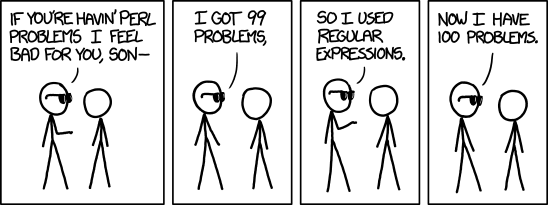
\includegraphics[width=10cm]{Chapters/04_perl_problems.png}
\end{center}
\caption{Regex XKCD\footnotemark}
\label{img:regex-xkcd}
\end{figure}

\footnotetext{Image from: http://xkcd.com/1171/}

\section{Matching an URI}
\label{sec:matching-an-uri}
So suppose we have the following line in our HTML file:
\begin{lstlisting}[
	language=html,
	tabsize=3,
	caption=Example line in HTML file,
	label=code:html-example,
	frame=shadowbox,
	rulesepcolor=\color{gray},
	xleftmargin=20pt,
	framexleftmargin=15pt,
	keywordstyle=\color{blue}\bf,
	commentstyle=\color{OliveGreen},
	stringstyle=\color{red},
	numbers=left,
	numberstyle=\tiny,
	numbersep=5pt,
	breaklines=true,
	showstringspaces=false,
	basicstyle=\footnotesize,
	emph={food,name,price},
	emphstyle={\color{magenta}}
]
<a href="http://www.google.com">
\end{lstlisting}

If you want to get the URI, you could use the following regular expression.
\begin{lstlisting}[
	tabsize=3,
	caption=Example regex,
	label=code:regex,
	frame=shadowbox,
	rulesepcolor=\color{gray},
	xleftmargin=20pt,
	framexleftmargin=15pt,
	keywordstyle=\color{blue}\bf,
	commentstyle=\color{OliveGreen},
	stringstyle=\color{red},
	numbers=left,
	numberstyle=\tiny,
	numbersep=5pt,
	breaklines=true,
	showstringspaces=false,
	basicstyle=\footnotesize,
	emph={food,name,price},
	emphstyle={\color{magenta}}
]
href=\"([^\"]+) "
\end{lstlisting}
There are some problems with this solution.
\begin{enumerate}
\item It would also capture \textit{href}
\item It would capture \textit{=}
\item And last but not at least, it would capture the quotes \textit{"}
\end{enumerate}
This is not what we want, since it would result in the matching of \textit{href="http://www.google.com"}. It is possible to solve this with lookarounds.

\section{Introducing lookarounds}
\label{sec:introducing-lookarounds}
Lookarounds, as the name might reveal, enforces something to be, or not to be, in front or after the expression. It is \textbf{not} part of the match. The only downside with lookarounds is that it is not included in every regex engine. It is also not POSIX compliant, but it works in PCRE, which is a very common regex engine (perl regex style).
\\
\\
The syntax is as follows:\\
\begin{table}
\begin{tabular}{l | l || p{5cm}}
Lookaround & Name & What it does \\ \hline
\texttt{(?=foo)} & Lookahead & Asserts that what immediately follows the current position in the string is foo \\ \hline
\texttt{(?<=foo))} & Lookbehind & Asserts that what immediately precedes the current position in the string is foo \\ \hline
\texttt{(?!foo)} & Negative Lookahead & Asserts that what immediately follows the current position in the string is not foo \\ \hline
\texttt{(?<!foo)} & Negative Lookbehind & Asserts that what immediately precedes the current position in the string is not foo \\ \hline
\end{tabular}
\caption{Table showing lookarounds \cite{regex-lookaround}}
\end{table}

\section{Using lookaround}
\label{sec:using-lookaround}
Now lets use the information from Section \ref{sec:introducing-lookarounds} and use this information to match the URI like we did in Section \ref{sec:matching-an-uri}.

We wanted to match the URL in the line below.
\begin{lstlisting}[
	language=html,
	tabsize=3,
	caption=Example line in HTML file,
	label=code:html-example-line,
	frame=shadowbox,
	rulesepcolor=\color{gray},
	xleftmargin=20pt,
	framexleftmargin=15pt,
	keywordstyle=\color{blue}\bf,
	commentstyle=\color{OliveGreen},
	stringstyle=\color{red},
	numbers=left,
	numberstyle=\tiny,
	numbersep=5pt,
	breaklines=true,
	showstringspaces=false,
	basicstyle=\footnotesize,
	emph={food,name,price},
	emphstyle={\color{magenta}}
]
<a href="http://www.google.com">
\end{lstlisting}
If we use lookahead and lookbehind, we can exactly match the URL. The regex below is an example that could be used.
\begin{lstlisting}[
	tabsize=3,
	caption=Example regex with lookahead and lookbehind,
	label=code:regex-lookbehind,
	frame=shadowbox,
	rulesepcolor=\color{gray},
	xleftmargin=20pt,
	framexleftmargin=15pt,
	keywordstyle=\color{blue}\bf,
	commentstyle=\color{OliveGreen},
	stringstyle=\color{red},
	numbers=left,
	numberstyle=\tiny,
	numbersep=5pt,
	breaklines=true,
	showstringspaces=false,
	basicstyle=\footnotesize,
	emph={food,name,price},
	emphstyle={\color{magenta}}
]
(?<=href=")([^"]+)(?=")
\end{lstlisting}
The regex above, using lookahead and lookbehind, will first look if there is a \textit{href="} in front of your expression. It will also look if there is a quote \textit{"} after your expression. If this is true, then it will match all characters except the quote \textit{"}. This will result in a match with exactly the URL. An example of what would match is given below.

\begin{lstlisting}[
	tabsize=3,
	caption=Example of the matched string,
	label=code:regex-match,
	frame=shadowbox,
	rulesepcolor=\color{gray},
	xleftmargin=20pt,
	framexleftmargin=15pt,
	keywordstyle=\color{blue}\bf,
	commentstyle=\color{OliveGreen},
	stringstyle=\color{red},
	numbers=left,
	numberstyle=\tiny,
	numbersep=5pt,
	breaklines=true,
	showstringspaces=false,
	basicstyle=\footnotesize,
	emph={food,name,price},
	emphstyle={\color{magenta}}
]
http://www.google.com
\end{lstlisting}
Please note that even the quotes are \textbf{not} matched.

\section{Greedy vs lazy}
\label{sec:greedy-vs-lazy}
Per default, your regex would be mostly greedy. To make it more clear we will provide the reader with an example. Lets say we want to \textbf{only} capture the HTML tags from the string below.

\begin{lstlisting}[
	language=html,
	tabsize=3,
	caption=Example regex with lookahead and lookbehind,
	label=code:html-example-string,
	frame=shadowbox,
	rulesepcolor=\color{gray},
	xleftmargin=20pt,
	framexleftmargin=15pt,
	keywordstyle=\color{blue}\bf,
	commentstyle=\color{OliveGreen},
	stringstyle=\color{red},
	numbers=left,
	numberstyle=\tiny,
	numbersep=5pt,
	breaklines=true,
	showstringspaces=false,
	basicstyle=\footnotesize,
	emph={food,name,price},
	emphstyle={\color{magenta}}
]
<p>test</p>
\end{lstlisting}
You can use the dot and certain quantifiers to match the tags. One way of doing it would be the following.
\begin{lstlisting}[
	language=html,
	tabsize=3,
	caption=Example regex with lookahead and lookbehind,
	label=code:regex-quantifiers,
	frame=shadowbox,
	rulesepcolor=\color{gray},
	xleftmargin=20pt,
	framexleftmargin=15pt,
	keywordstyle=\color{blue}\bf,
	commentstyle=\color{OliveGreen},
	stringstyle=\color{red},
	numbers=left,
	numberstyle=\tiny,
	numbersep=5pt,
	breaklines=true,
	showstringspaces=false,
	basicstyle=\footnotesize,
	emph={food,name,price},
	emphstyle={\color{magenta}}
]
/<.+>/g
\end{lstlisting}
However, this method would match everything like below.

\begin{lstlisting}[
	language=html,
	tabsize=3,
	caption=Example regex with lookahead and lookbehind,
	label=code:regex-match-quantifiers,
	frame=shadowbox,
	rulesepcolor=\color{gray},
	xleftmargin=20pt,
	framexleftmargin=15pt,
	keywordstyle=\color{blue}\bf,
	commentstyle=\color{OliveGreen},
	stringstyle=\color{red},
	numbers=left,
	numberstyle=\tiny,
	numbersep=5pt,
	breaklines=true,
	showstringspaces=false,
	basicstyle=\footnotesize,
	emph={food,name,price},
	emphstyle={\color{magenta}}
]
<p>test</p>
\end{lstlisting}
One way to overcome is to use the question mark (\textit{?}), which specifies that this part of the regex should be lazy. It would result in the following regex.
\begin{lstlisting}[
	language=html,
	tabsize=3,
	caption=Example regex with lookahead and lookbehind,
	label=code:regex-lookaround,
	frame=shadowbox,
	rulesepcolor=\color{gray},
	xleftmargin=20pt,
	framexleftmargin=15pt,
	keywordstyle=\color{blue}\bf,
	commentstyle=\color{OliveGreen},
	stringstyle=\color{red},
	numbers=left,
	numberstyle=\tiny,
	numbersep=5pt,
	breaklines=true,
	showstringspaces=false,
	basicstyle=\footnotesize,
	emph={food,name,price},
	emphstyle={\color{magenta}}
]
/<.+?>/g
\end{lstlisting}
Here we would match just the HTML tags. Please note, since we have set the global quantifiers, it would match both tags. The example below would present the reader with what would be matched.

\begin{lstlisting}[
	language=html,
	tabsize=3,
	caption=Example regex with lookahead and lookbehind,
	label=code:regex-lookaround2,
	frame=shadowbox,
	rulesepcolor=\color{gray},
	xleftmargin=20pt,
	framexleftmargin=15pt,
	keywordstyle=\color{blue}\bf,
	commentstyle=\color{OliveGreen},
	stringstyle=\color{red},
	numbers=left,
	numberstyle=\tiny,
	numbersep=5pt,
	breaklines=true,
	showstringspaces=false,
	basicstyle=\footnotesize,
	emph={food,name,price},
	emphstyle={\color{magenta}}
]
<p></p>
\end{lstlisting}
As you can see, both \textcolor{red}{\texttt{<p>}} and \textcolor{green}{\texttt{</p>}} would be matched.

\section{Word boundary}
\label{sec:word-boundary}
There could also be a use case where you want to match a specific word using regex. In this use case we assume that you want to only match a whole word (without any characters in front or behind that specific word). One way of using regex in this certain use case is the use of word boundaries. The following regex is using this word boundary to match the word (\textit{example}).

\begin{lstlisting}[
	language=html,
	tabsize=3,
	caption=Example regex with lookahead and lookbehind,
	label=code:regex-word-boundary,
	frame=shadowbox,
	rulesepcolor=\color{gray},
	xleftmargin=20pt,
	framexleftmargin=15pt,
	keywordstyle=\color{blue}\bf,
	commentstyle=\color{OliveGreen},
	stringstyle=\color{red},
	numbers=left,
	numberstyle=\tiny,
	numbersep=5pt,
	breaklines=true,
	showstringspaces=false,
	basicstyle=\footnotesize,
	emph={food,name,price},
	emphstyle={\color{magenta}}
]
/\bexample\b/g
\end{lstlisting}
\label{exmp:word-boundarie-regex}

If use it against the string below, it would match nothing.
\begin{lstlisting}[
	language=html,
	tabsize=3,
	caption=Example regex with lookahead and lookbehind,
	label=code:regex-match-word-boundary,
	frame=shadowbox,
	rulesepcolor=\color{gray},
	xleftmargin=20pt,
	framexleftmargin=15pt,
	keywordstyle=\color{blue}\bf,
	commentstyle=\color{OliveGreen},
	stringstyle=\color{red},
	numbers=left,
	numberstyle=\tiny,
	numbersep=5pt,
	breaklines=true,
	showstringspaces=false,
	basicstyle=\footnotesize,
	emph={food,name,price},
	emphstyle={\color{magenta}}
]
examples
\end{lstlisting}
It can not match the word example, since there is an \textit{'s'} after the word \textit{example}. With word boundaries the word must be free \textit{(i.e., there can not be any characters in front of after it)}.

Let's assume the following string.
\begin{lstlisting}[
	language=html,
	tabsize=3,
	caption=Example regex with lookahead and lookbehind,
	label=code:regex-example-string,
	frame=shadowbox,
	rulesepcolor=\color{gray},
	xleftmargin=20pt,
	framexleftmargin=15pt,
	keywordstyle=\color{blue}\bf,
	commentstyle=\color{OliveGreen},
	stringstyle=\color{red},
	numbers=left,
	numberstyle=\tiny,
	numbersep=5pt,
	breaklines=true,
	showstringspaces=false,
	basicstyle=\footnotesize,
	emph={food,name,price},
	emphstyle={\color{magenta}}
]
This is an example with a match
\end{lstlisting}
If we would use the regex with the word boundaries, it would match the exact word \textit{example}. The word does not contain any other characters than the \textbf{exact same word} in the regex. Hence why we this time have a match.
